% Chapter 3: Methodology

This chapter describes the methods and approaches used in the experiments. This includes the selection of dataset, models, loss functions, as well as training and evaluation strategies.

\section{Overview of Approach}

Image classification involves predicting the correct category of an image from a set of predefined classes. This project focuses on addressing the challenge of class imbalance, where some classes have many samples while others have very few.

The CIFAR-100 dataset \cite{krizhevsky2009learning} was chosen because it is small enough to work with efficiently and is commonly used in other research. To create a long-tailed version of the dataset, its class distribution was adjusted to match the distribution of the ImageNet-LT dataset used in \cite{zhang2023deep}. This adjustment ensures that the experiments simulate real-world class imbalance.

Several loss functions designed to handle class imbalance were tested in this project, including Softmax Cross-Entropy (CE), Focal Loss (FL), Class-Balanced (CB) Loss, Balanced Softmax (BS) Loss, Equalization (EQ) Loss, and LDAM Loss. These loss functions modify how the models learn, making it easier for them to focus on classes with fewer samples.

The experiments were performed using four model architectures: ResNet50, MobileNetV2, ConvNeXt Base, and ViT-B/16. All models were pretrained on ImageNet, which provided a strong starting point for fine-tuning on the CIFAR-100 dataset. These models were chosen because they are well-suited for image classification tasks and represent different design approaches.

Each model was trained on both a balanced training set and a long-tailed training set. The performance of the models was evaluated using a balanced test set, a long-tailed test set, and the long-tailed test set divided into head, middle, and tail classes. This division made it possible to analyze the performance for classes with different numbers of samples. The main evaluation metric used was top-1 accuracy, which measures how often the model's top prediction is correct.

In what follows, each step of the methodology will be explained in detail.

\section{Dataset Preparation and Specifications}
\label{sec:dataset_specs}
A description of this section here.

Following the dataset structure used in \textit{Deep Long-Tailed Learning: A Survey}, the CIFAR100 dataset was modified to create a long-tailed training set and a balanced test set. 

\subsection{Benchmark Dataset Selection}
There are a number of benchmark datasets for long-tailed image classification tasks, including ImageNet-LT, Places365-Lt, CIFAR-100-LT, and iNaturalist 2018 \todo{references}. The previous three are sampled from ImageNet, Places365, and CIFAR-100, following the Pareto distribution, as described in section \ref{sec:lt-datasets}, while the iNaturalist 2018 is a natural long-tailed dataset. Table \ref{tab:datasets} summarizes the four datasets and their data specifications. 

\begin{table}[ht]
    \centering
    \caption{Summary of long-tailed benchmarks for image classification. \todo{references}}
    \begin{tabular}{lccc}
    \hline
    \textbf{Dataset}           & \textbf{\# Classes} & \textbf{\# Training Data} & \textbf{\# Test Data} \\ \hline
    ImageNet-LT   & 1,000              & 115,846                   & 50,000                \\
    CIFAR100-LT   & 100                & 50,000                    & 10,000                \\
    Places-LT     & 365                & 62,500                    & 36,500                \\
    iNaturalist 2018 & 8,142            & 437,513                   & 24,426                \\ \hline
    \end{tabular}
    \label{tab:datasets}
\end{table}
    

With its 100 classes and only 60,000 samples, the CIFAR-100 dataset was chosen as a benchmark for the experiments conducted in this thesis based on its managable size, compared to the other benchmarks, and widespread use as a standard in image classification research \todo{reference}. It's comparatively small size allows for rapid experimentation and comparisons, wheras a larger benchmark requires more computational effort and time for experiments, thus it is well-suited for multiple configurations and evaluations. However, CIFAR-100 has some limitations comparet to larger dataset, like ImageNet-LT or iNaturalist. For example, CIFAR-100 images are of relatively low resolution ($32 \times 32$ pixels) compared to ImageNet ($224 \times 224$ pixels), and may limit the ability of models to capture fine-grained details. Likewise, the smaller number of classes and samples can result in less diversity compared to datasets like iNaturalist 2018, which contains nearly nine times as many samples in the training data as CIFAR-100-LT. Despite these drawbacks, CIFAR-100-LT remains a practical choice for this thesis due to its computational efficiency. 

\todo{Describe the type of images in CIFAR-100 and include examples.}

\subsection{Data Characteristics: Class Distribution}
Understanding the class distribution in long-tailed datasets is essential for evaluating the impact of the class imbalance on model performance. This section analyzes the class distribution of the benchmark ImageNet-LT used in \cite{zhang2023deep}, which serves as a reference for creating a similar distribution across the CIFAR-100-LT training, evaluation, and test datasets.  

The ImageNet-LT dataset, introduced by Liu et al. \cite{liu2019largescalelongtailedrecognitionopen}, has been widely used in empirical studies, including \textit{Deep Long-Tailed Learning: A Survey} \cite{zhang2023deep}. The class distributions of its training, validation, and test sets are shown in Figures~\ref{fig:IN-train}, \ref{fig:IN-val}, and \ref{fig:IN-test}, respectively. The ImageNet-LT is constructed from the original ImageNet-2012 following the Pareto-distribution (Eq. \eqref{eq:pareto}) with power value $\alpha=6$ \cite{liu2019largescalelongtailedrecognitionopen}, resulting in an imbalance ratio of 256, meaning that the most frequent class has 256 times more samples than the least frequent class. As suggested in figure \ref{fig:IN-train}, the most frequent class has 1280 images, and the least frequent class 5 images \cite{liu2019largescalelongtailedrecognitionopen}. The power value of 6 is relatively large, resulting in the steep imbalance and very few samples in the tail, as seen in figure \ref{fig:IN-train}. The underrepresentation in the tail classes poses a significant challenge for models to learn from tail classes. Both the validation and test sets are balanced, as shown in figures \ref{fig:IN-val} and \ref{fig:IN-test}, respectively. There are 20 samples per class in the validation set, and 50 samples per class in the test set. \todo{remove the figures, and just leave it in writing.}


\begin{figure}[h!]
    \centering
    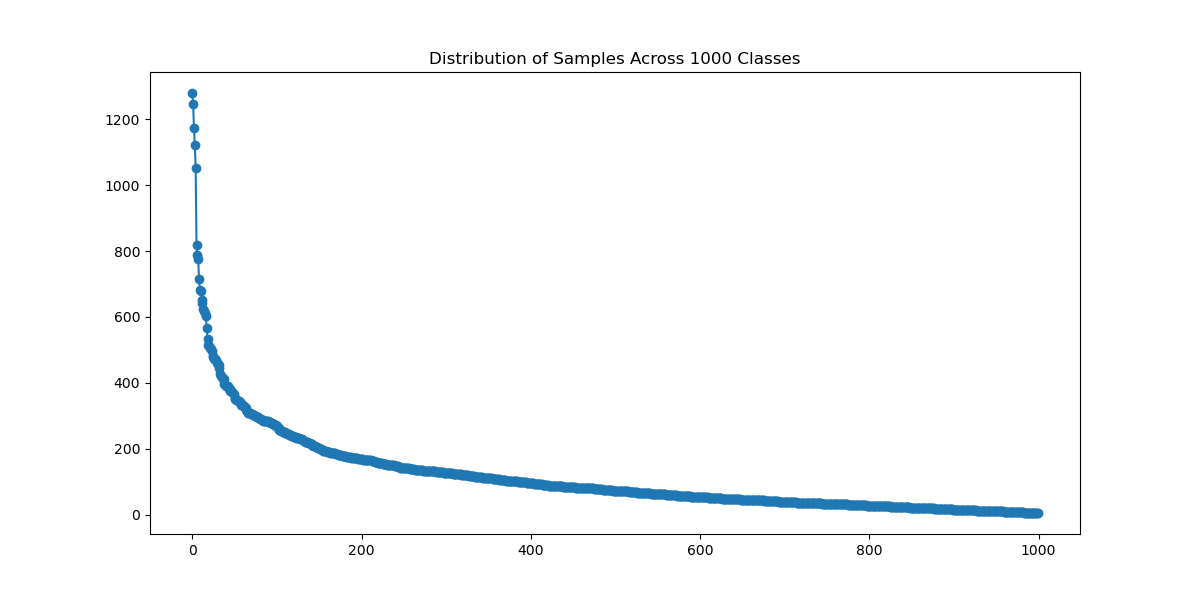
\includegraphics[width=0.9\textwidth]{Images/Plots/class_distribution_train.png}
    \caption{The class distribution of the training images for the ImageNet-LT dataset shows a long-tailed distribution.}
    \label{fig:IN-train}
\end{figure}

% \begin{figure}[h!]
%     \centering
%     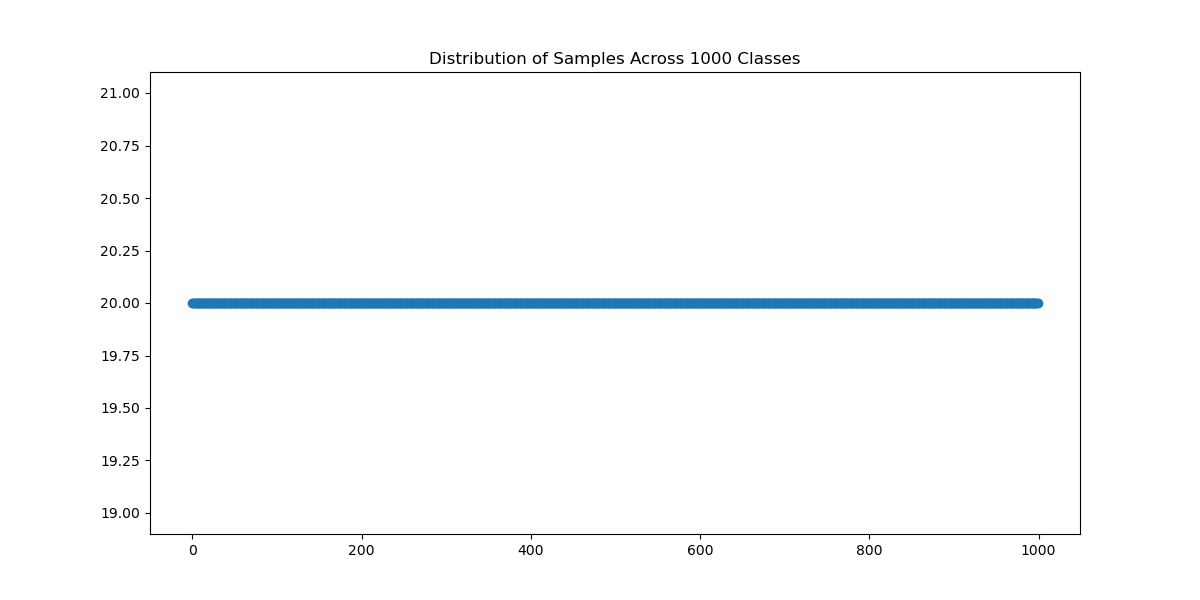
\includegraphics[width=0.9\textwidth]{Images/Plots/class_distribution_val.png}
%     \caption{The class distribution of the validation images for the ImageNet-LT dataset shows that there are 20 samples of each class.}
%     \label{fig:IN-val}
% \end{figure}

% \begin{figure}[h!]
%     \centering
%     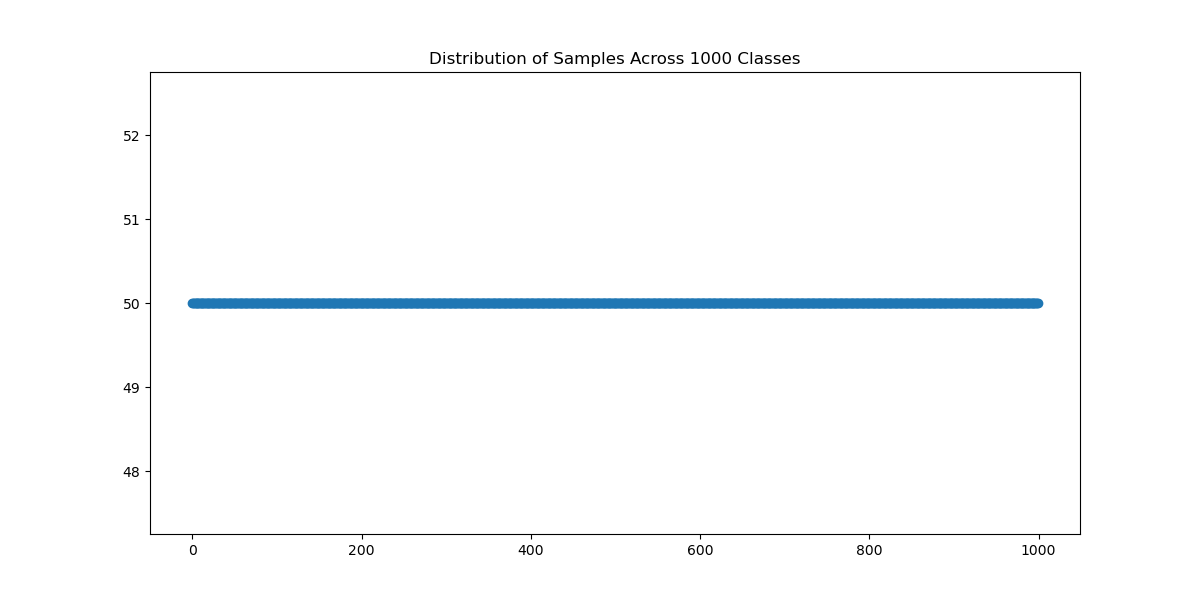
\includegraphics[width=0.9\textwidth]{Images/Plots/class_distribution_test.png}
%     \caption{The class distribution of the test images for the ImageNet-LT dataset shows that there are 50 samples of each class.}
%     \label{fig:IN-test}
% \end{figure}


However, investigating the CIFAR-100-LT dataset used in \emph{Learning Imbalanced Datasets with Label-Distribution-Aware Margin Loss} by Cao et al. \cite{cao2019learningimbalanceddatasetslabeldistributionaware} shows that the training dataset follows a exponential decay, and not a pareto distribution. The imbalance factor in their studies is 100, meaning that the most frequent class has 100 times more samples than the least frequent class, following equation \eqref{eq:exp}. This means that the imbalance is not as steep as with the Pareto distribution, resulting in a middle section of classes with fewer samples than the head classes, but more samples than the tail classes, see figure \ref{fig:cifar100_train_450_imb}. The following section will describe the preparation of CIFAR-100 for the experiments in this thesis.


\subsection{CIFAR-100-LT}
The experiments conducted in this thesis are trained and evaluated on the CIFAR-100 dataset. This was downloaded using the PyTorch torchvision.datasets.CIFAR100 \cite{pytorch_cifar100}. The training and test datasets were preprocessed by converting the images to tensors using the ToTensor transformation and saved as .pth files for efficient loading during experiments. 

The class distributions used in experiments in this thesis: Balanced training set, balanced test set, balanced validation set, long-tailed training set, long-tailed test set, long-tailed test set split into head, middle and tail. The class distributions can be seen in table \ref{tab:class_distributions}.

\begin{table}[h!]
    \centering
    \caption{Class Distributions Used in Experiments}
    \label{tab:class_distributions}
    \begin{tabular}{|l|c|}
    \hline
    \textbf{Dataset Type}                       & \textbf{Samples}                                                                 \\ \hline
    Balanced Training Set                       & 45,000        \\ \hline
    Balanced Validation Set                     & 10,000    \\ \hline
    Balanced Test Set                           & 5,000    \\ \hline
    Long-Tailed Training Set                    & \todo{-}      \\ \hline
    Long-Tailed Test Set                        & \todo{-} \\ \hline
    Head  & \todo{-} \\ \hline
    Middle   & \todo{-} \\ \hline
    Tail  & \todo{-} \\ \hline
    \end{tabular}
    \end{table}
    

To address the needs of the experiments in this thesis, the original CIFAR-100 dataset was modified to create a new split from the training data. Specifically, the training data was split into 450 samples per class for training and 50 samples per class for testing, mirroring the test data for the ImageNet. The original test set of the CIFAR-100 dataset was retained as the validation set for evaluation during training. All datasets were saved locally to maintain reproducibility.

% \begin{figure}[h!]
%     \centering
%     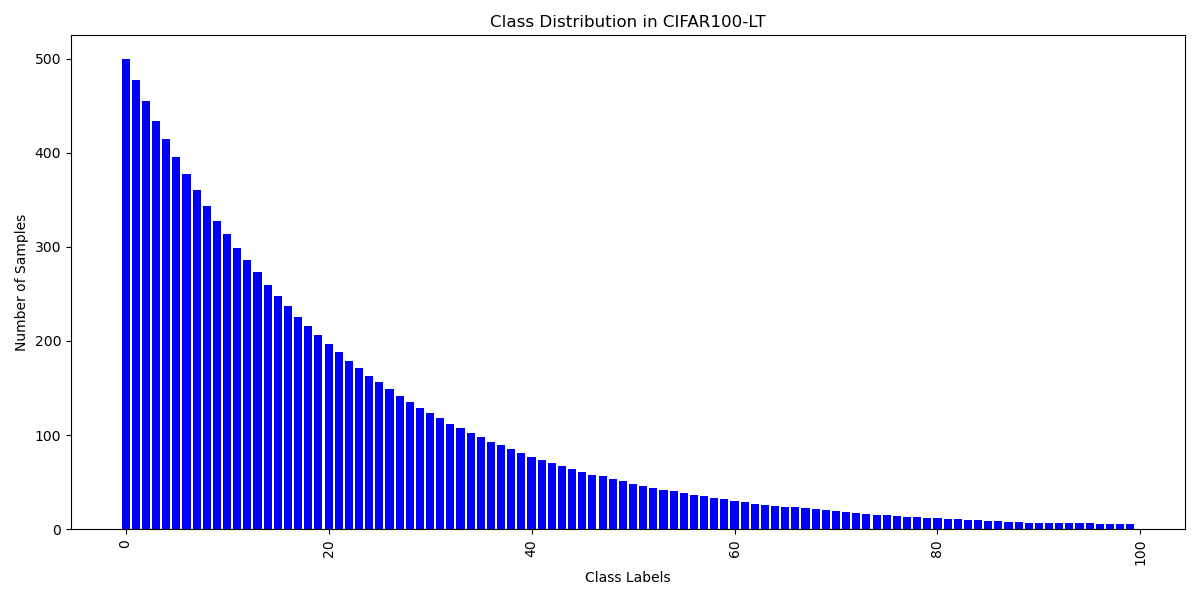
\includegraphics[width=0.9\textwidth]{Images/Plots/Class Distribution for CIFAR100-LT.png}
%     \caption{The class distribution of CIFAR100-LT with imbalance ratio 100 generated by the imbalance\_cifar.py in the LDAM-DRW GitHub repository \cite{kaidic_ldam_drw}.}
%     \label{fig:cifar100_imbalance_cifar}
% \end{figure}

% \begin{figure}[h!]
%     \centering
%     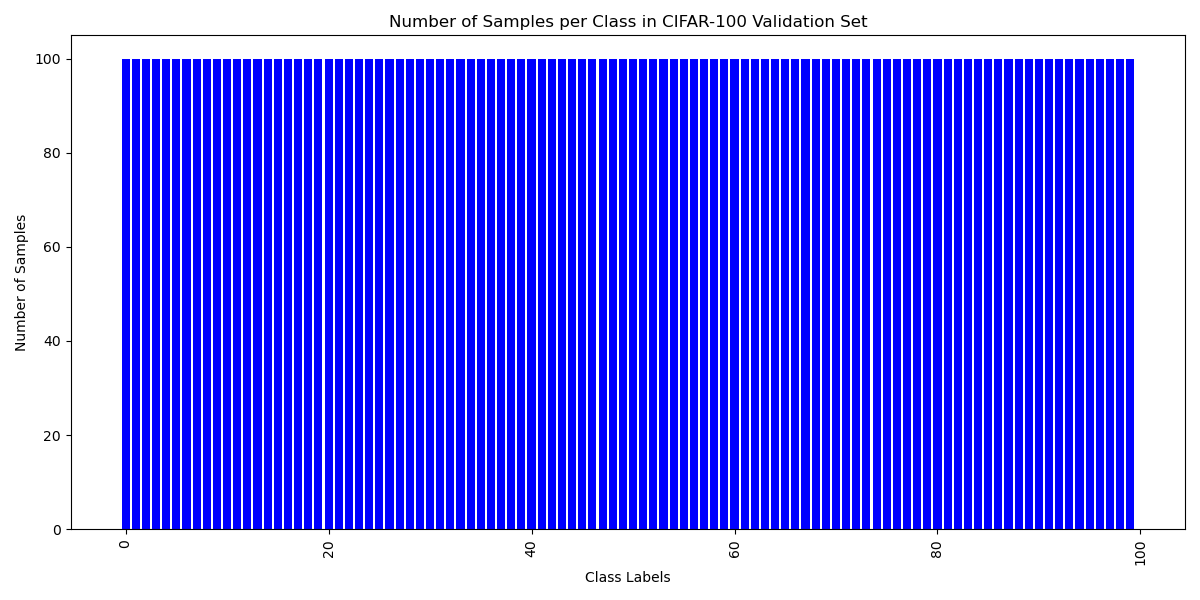
\includegraphics[width=0.9\textwidth]{Images/Plots/cifar100_val_class_distribution.png}
%     \caption{The class distribution of the CIFAR100 validation set from torchvision \cite{pytorch_cifar100}.}
%     \label{fig:cifar100val}
% \end{figure}

\textbf{Long-tailed Training Set:} To simulate real-world scenarios with class imbalances, the training dataset was modified to introduce an exponential imbalance across the 100 classes. Following the procedure of \cite{cao2019learningimbalanceddatasetslabeldistributionaware}, the imbalance was created using exponential decay. Here, the number of samples per class decreases exponentially, controlled by the imbalance factor, following equation \eqref{eq:exp}. For this thesis, an imbalance factor of 100 was applied. This means that the most frequent class contains a 100 times more samples than the least frequent class. 

\begin{figure}[h!]
    \centering
    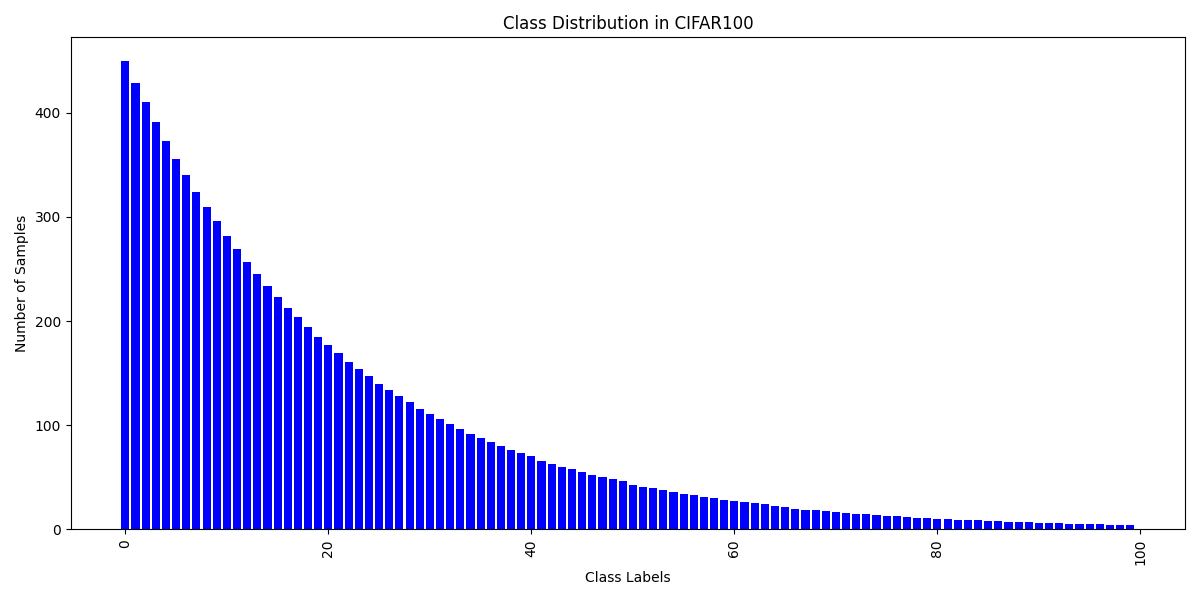
\includegraphics[width=0.9\textwidth]{Images/Plots/cifar100_train_450_imb.png}
    \caption{The class distribution of the CIFAR-100 long-tailed training set with 450 samples in the most frequent class.}
    \label{fig:cifar100_train_450_imb}
\end{figure}

The resulting class distribution varied from the most frequent class having 450 samples to the least frequent class having only 4 samples, as shown in figure \ref{fig:cifar100_train_450_imb}. This imbalance ensured no class was left with zero samples, maintaining the integrity of all classes for training. The dataset was saved locally to maintain reproducibility.


\textbf{Long-Tailed Test Set:} To evaluate the performance of the model under similar conditions to the imbalanced training set, an imbalanced test set was created from the previously split test dataset. The imbalance in the test set mirrors the exponential distribution used for the training data, with the same imbalance factor of 0.01. The class distribution in the test set follows the same order of classes (from most to least frequent) as the imbalanced training set. No class has fewer than one sample. The class distribution can be seen in figure \ref{fig:cifar100_test_imb}. The dataset was saved locally to maintain reproducibility.

% \begin{figure}[h!]
%     \centering
%     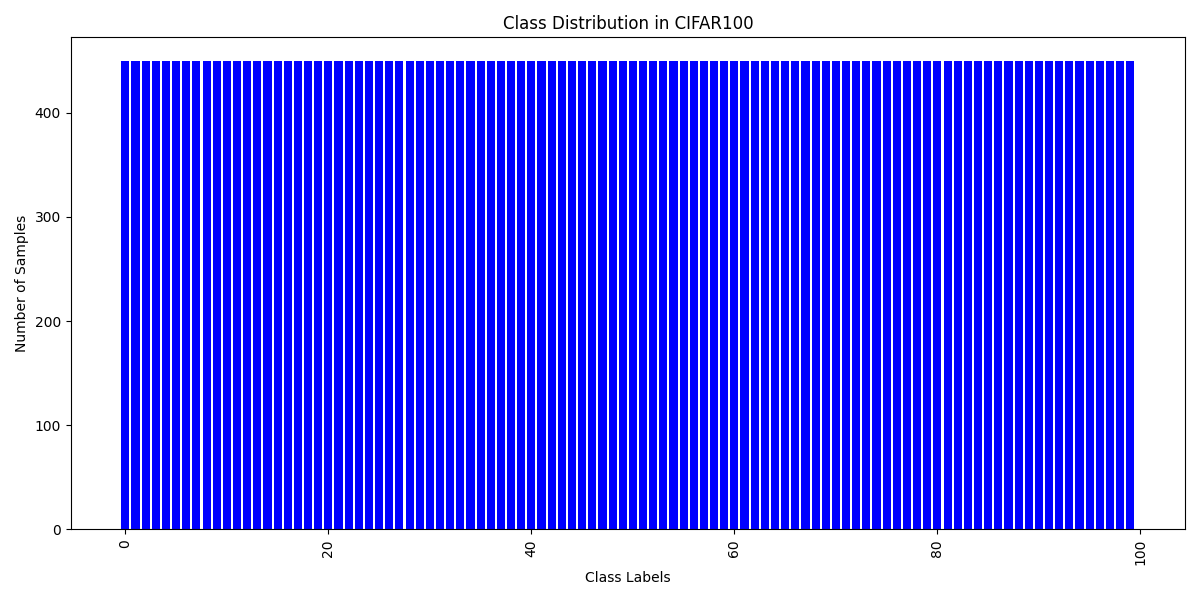
\includegraphics[width=0.9\textwidth]{Images/Plots/cifar100_bal_train_450.png}
%     \caption{The class distribution of the CIFAR-100 balanced training set with 450 samples per class.}
%     \label{fig:cifar100_train_450}
% \end{figure}

\begin{figure}[h!]
    \centering
    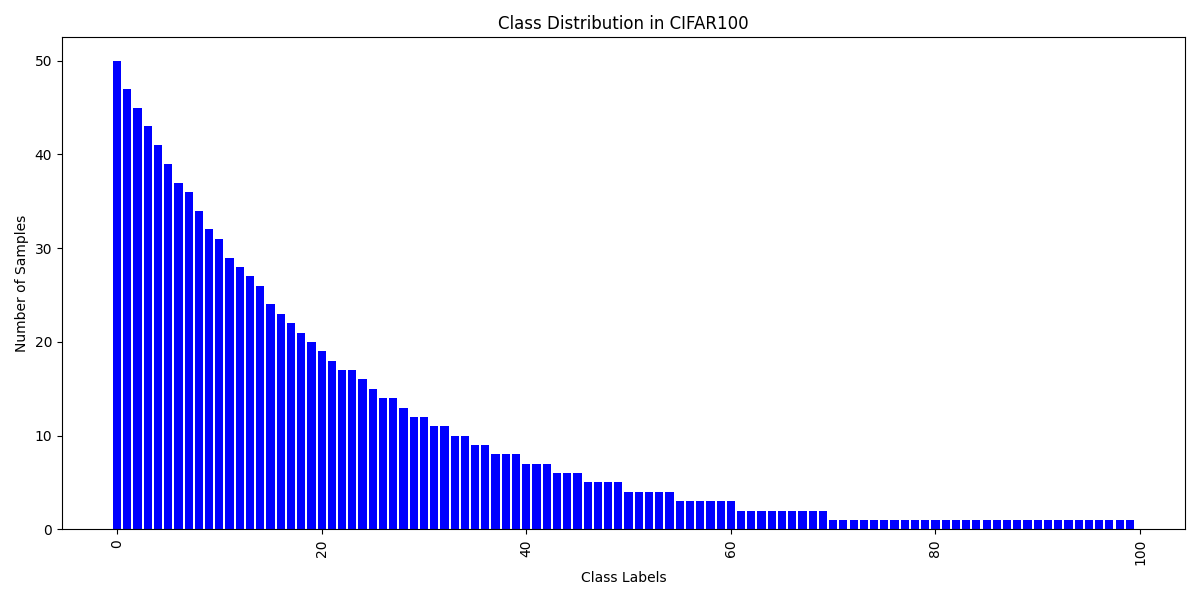
\includegraphics[width=0.9\textwidth]{Images/Plots/cifar100_test_imb.png}
    \caption{The class distribution of the CIFAR-100 long-tailed test set with 50 samples in the most frequent class.}
    \label{fig:cifar100_test_imb}
\end{figure}

To further analyze performance, the test set was divided into three subsets: head, middle, and tail classes. The head classes comprised the top 33\% most frequent classes, the middle classes included the next 33\%, and the tail classes represented the bottom 33\%. See table \ref{tab:class_distributions}. This categorization allows for a detailed evaluation of the methods across different classes. 


% \begin{figure}[h!]
%     \centering
%     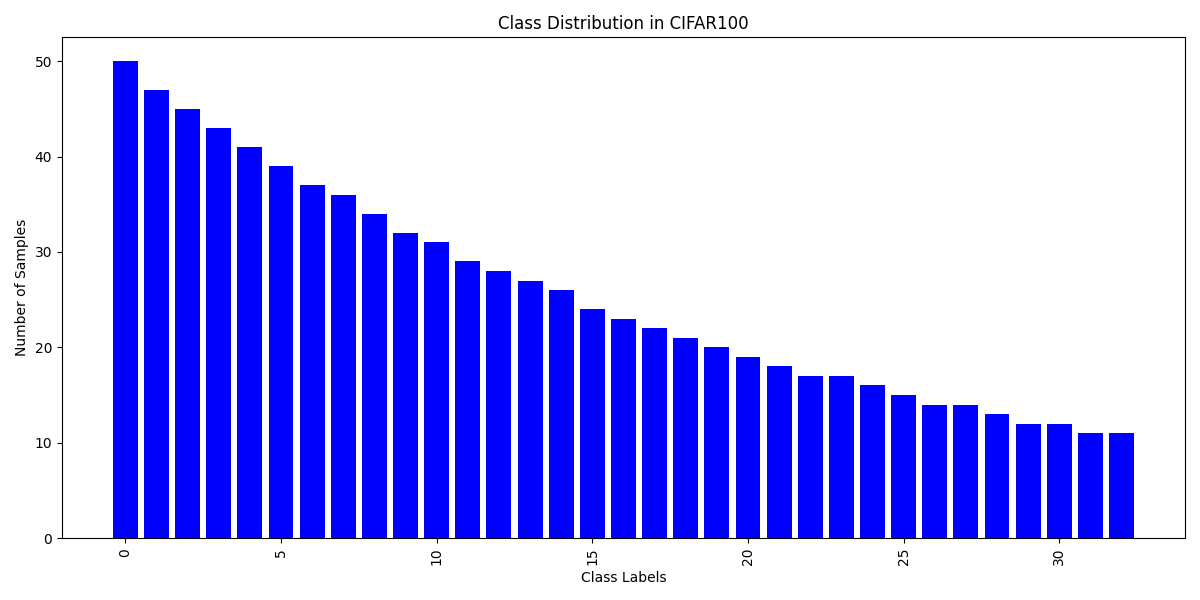
\includegraphics[width=0.9\textwidth]{Images/Plots/cifar100_test_head.png}
%     \caption{The class distribution of the CIFAR-100 long-tailed test head classes.}
%     \label{fig:cifar100_test_head}
% \end{figure}


% \begin{figure}[h!]
%     \centering
%     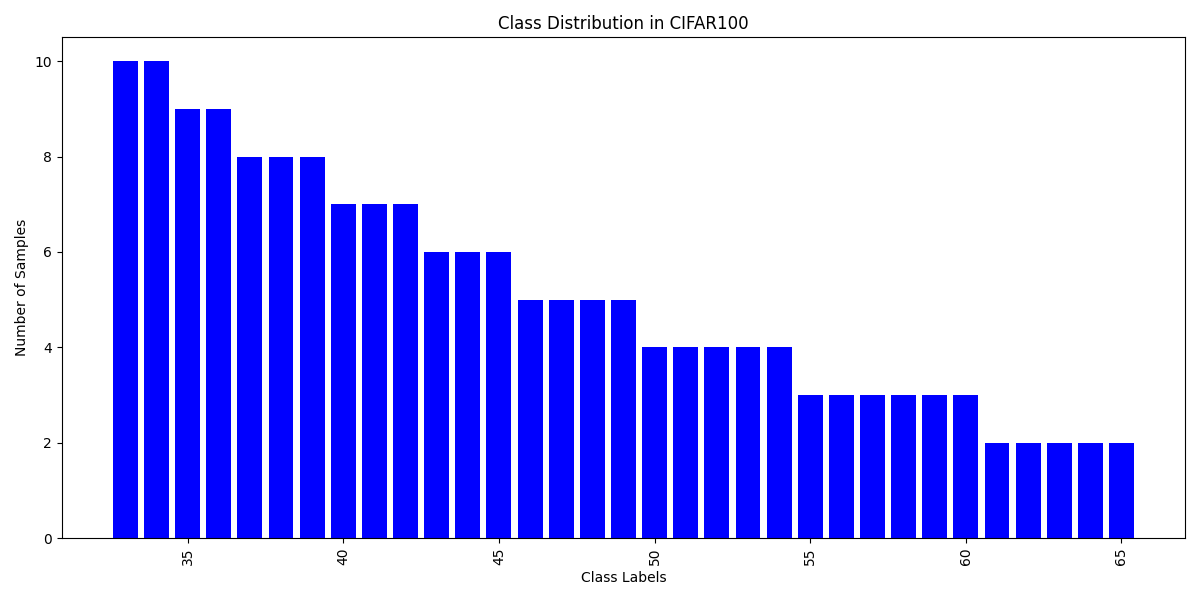
\includegraphics[width=0.9\textwidth]{Images/Plots/cifar100_test_middle.png}
%     \caption{The class distribution of the CIFAR-100 long-tailed test middle classes.}
%     \label{fig:cifar100_test_middle}
% \end{figure}

% \begin{figure}[h!]
%     \centering
%     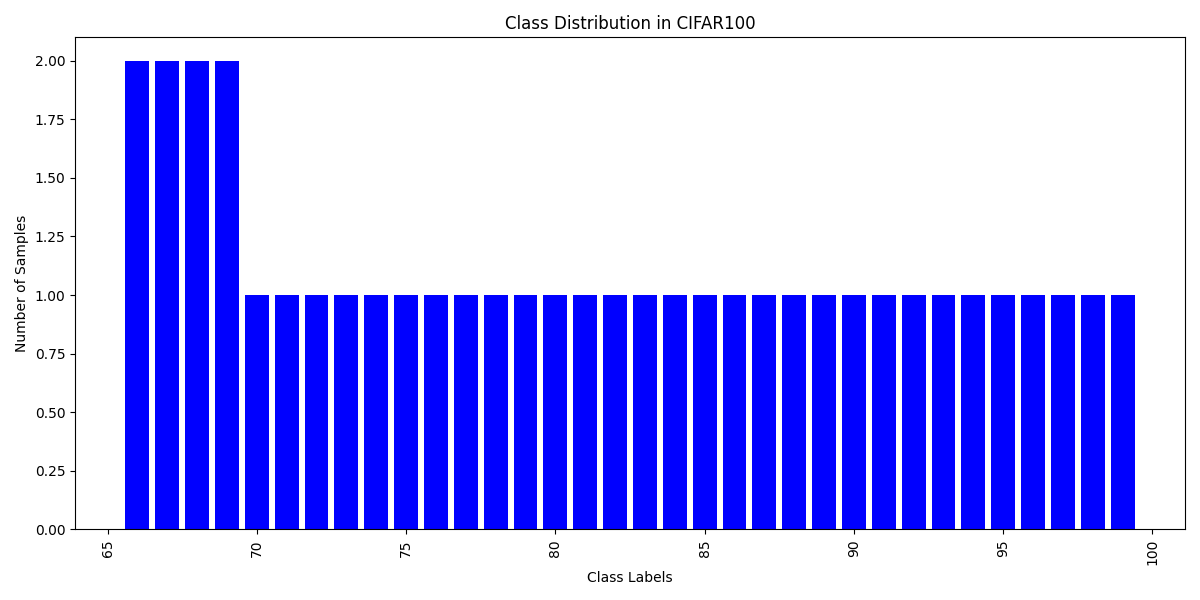
\includegraphics[width=0.9\textwidth]{Images/Plots/cifar100_test_tail.png}
%     \caption{The class distribution of the CIFAR-100 long-tailed test tail classes.}
%     \label{fig:cifar100_test_tail}
% \end{figure}


\subsection{Data Augmentation}
Data augmentation and normalization were applied to the CIFAR-100 dataset to improve the generalization capability of the models. For the CIFAR-100 dataset, the augmentations were applied using the CIFAR-100 RGB statistics, with mean values [0.4914, 0.4822, 0.4465], and standard deviations [0.2023, 0.1994, 0.2010] \cite{kaidic_ldam_drw}. These values are used to normalize the images after applying the transformations. However, the models used in this study are all pretrained on ImageNet, and choosing the ImageNet RGB statistics could potentially influence the training, as the pretrained weights are optimized for inputs with ImageNet statistics. Future work could explore the impact of using ImageNet statistics instead.

Images were resized to 224x224 pixels to match the input requirements of the ImageNet-pretrained models. Random cropping with a padding of 4 was applied to introduce spatial variations, while horizontal flipping with a 50\% probability further augmented the data. After these transformations, images were normalized using the CIFAR-100-specific mean and standard deviation values, ensuring consistency with the dataset.

For validation, a simpler approach was used, where images were resized to 224x224 pixels and normalized using the same mean and standard deviation values as the training set.

\section{Long-tailed Learning Techniques}
This section outlines the methods employed to address the challenges posed by a long-tailed data distribution. Specifically, it discusses the choice of model architecture and class re-balancing methods, including their strengths, limitations, and rationale based on prior research and feasible implementations.  

\subsection{Model Selection}
\label{sec:model_selection}
% \textit{A list of subjects to include in this section:}

% \begin{itemize}
%     \item Mention the model architectures chosen for training, and describe why they are appropriate for deep long-tailed learning with reference to the background section.
%     \item Discuss the strengths and limitations of these models in addressing the challenges posed by imbalanced data.
%     \item Describe how they were pretrained (ImageNet-1K, ImageNet-21K) and what that means for the training on CIFAR100.
%     \item Write about their implementation. The implementation is the same for all models. 
%     \item Include the training loss for both balanced and imbalanced data.
%     \item Compare to the results in their original paper. 
% \end{itemize}

This section will discuss the choice of model architectures addressing the challenges of long-tailed datasets. The models evaluated in this thesis are four common state-of-the-art (SOTA) models: ResNet-50, MobileNetV2, ViT-B/16, and ConvNeXt-Base. These SOTA models were selected to represent a diverse range of architectures for solving image classification tasks and to pose a balance between computational efficiency and state-of-the-art performance. The models were modified and trained using transfer learning with pre-trained weights from ImageNet \cite{ILSVRC15}. Model complexity can be viewed in table \ref{tab:model_performance}.

For all models, the fully connected layer is modified to accomodate for the CIFAR-100 dataset's 100 classes.

Transfer learning:
\url{https://www.kaggle.com/code/riteshsinha/transfer-learning-using-resnet}
% Transfer learning enables pre-trained CNNs to adapt to new
% tasks with smaller datasets, a technique that has proven
% successful in fields ranging from medical imaging to
% environmental monitoring [14, 15, 26].
% In flower classification, transfer learning allows models
% trained on datasets like ImageNet to retain generalized
% features, enabling high classification accuracy with limited
% data. Studies like demonstrated over 90% accuracy on flower
% classification tasks using CNN-based transfer learning with
% fusion descriptors [20]. This study builds on these findings by
% applying transfer learning with ResNet-50 to a diverse dataset
% of flower images, evaluating its effectiveness in distinguishing
% among species with similar visual features.

Transfer learning, as briefly described in section \todo{write this}, leverages pre-trained neural networks to adapt to new tasks on smaller datasets, a method successfully applied in domains such as medical imaging and environmental monitoring \cite{pan2010,Hinton2006,Fu2021}. By utilizing models pre-trained on large-scale datasets like ImageNet, transfer learning allows for the retention of generalized features, enabling high performance even with limited data. In the context of this project, transfer learning is employed to evaluate its effectiveness in addressing the challenges of long-tailed datasets, specifically by enabling the model to generalize well across classes with varying sample sizes.


Fine-tuning: 
\url{https://medium.com/@caterine/fine-tuning-a-model-using-pytorch-part-2-e86a548ac4fb}
\url{https://www.tensorflow.org/tutorials/images/transfer_learning}

\begin{table}[ht]
    \centering
    \caption{Models. \todo{caption}}
    \scriptsize
    \begin{tabular}{lcccc}
    \toprule
    \textbf{Model} & \textbf{Type} & \textbf{Pre-trained} & \makecell{\textbf{Parameters} \\ \textbf{(millions)}} & \textbf{top-1 accuracy} \\
    \midrule
    MobileNetV2 \cite{sandler2018mobilenetv2} & CNN  & ImageNet-1K & - & 72.154 \cite{pytorch_mobilenetv2} \\
    ResNet50 \cite{he2015deepresiduallearningimage} & CNN & ImageNet-1K & - & 	
    80.858 \cite{torchvision-resnet} \\
    ConvNeXt-Base \cite{todi2023convnext}  & CNN & ImageNet-1K & 88.591.464 & 84.062 \cite{torchvision-convnext} \\
    ViT-B/16 \cite{dosovitskiy2021imageworth16x16words}   & ViT & \makecell{ImageNet-21K \\ (ft on ImageNet-1K)} & - & 	- \\
    \bottomrule
    \end{tabular}
    \label{tab:model_performance}
\end{table}

% We have selected and evaluated seven common state-of-the-art (SOTA) CNN models: ConvNext (Tiny and Base) (Todi et al., 2023), DenseNet121 (Huang et al., 2017), EfficientNetB4 (Tan and Le, 2019), InceptionV3 (Szegedy et al., 2016), MobileNetv2 (Sandler et al., 2018) and ResNet50v2 (He et al., 2016).
% The SOTA models were modified and trained using transfer learning with pre-trained weights from ImageNet (Russakovsky et al., 2015). Transfer learning involves training a model on data from a source domain 200 TS = P(y|X) and then transferring it to a target domain TT = P(y|X) – typically with less data available.
% In this case, ImageNet contains 1,000 classes with 1,281,167 images for training and 50,000 for testing, while the arthropod dataset only contains 19 classes with 13,812 images. For all models, a fully connected layer with a dropout rate of 0.2 was added and trained on the dataset, followed by fine-tuning of all base CNN layers.

\paragraph{ResNet-50}
Resnet-50 \cite{he2015deepresiduallearningimage} is a convolutional neural network designed with residual connections to mitigate the vanishing gradient problem, as detailed in section \ref{sec:resnet}. Introduced by He et al. in 2015, the ResNet architecure achieved unprecedented results and won ILSVRC 2015 for image classification tasks \cite{ILSVRC15}. 

With 50 layers, ResNet-50 strikes a balance between model complexity and computational efficiency. It is highly effective for extracting robust features, making it well-suited for image classification on long-tailed datasets \cite{he2015deepresiduallearningimage}. ResNet-50 has been utilized in various domains of image classification, including tasks such as medical imaging \cite{huang2022identifyingkeycomponentsresnet50, Simegn} and face detection \cite{Nyarko2022}, and commonly serves as a baseline in research \cite{yun2019cutmixregularizationstrategytrain,cubuk2019randaugmentpracticalautomateddata,zhang2018mixupempiricalriskminimization,menon2021longtaillearninglogitadjustment}. Leveraging pretrained weights on ImageNet-1K, it achieves better generalization on unseen datasets \cite{resnettransfer,RAZAVI2024123276,chan2019transfer,Shafiq2022}, with its top-1 accuracy shown in Table \ref{tab:model_performance}. 

Compared to smaller architectures like ResNet-16 and ResNet-34, ResNet-50 offers improved feature extraction while being more memory-efficient and faster to train than larger versions, such as ResNet-101 and ResNet-152 \cite{he2015deepresiduallearningimage}. This balance of performance and efficiency makes it suitable for smaller datasets like CIFAR-100 \cite{10083966}.

Chosen as a reference point for CNN designs in this study, ResNet-50 demoonstrate the advantages of transfer learning and remains a reliable choice for addressing class imbalance effectively. Its demonstrated versatility across various datasets underscores its value for robust image classification tasks \cite{he2015deepresiduallearningimage,yun2019cutmixregularizationstrategytrain,}.

\paragraph{MobileNetV2}
The MobileNetV2 model  is a successor to the ResNet architecture, adjusted to run on mobile devices. It requires fewer computational resources due to the introduction of inverted residual blocks and depthwise separable convolutions, as described in section \ref{sec:mobilenet}. This architecture was chosen to represent an example of a modern and lightweight CNN architecture that has achieved state-of-the-art performance \cite{sandler2018mobilenetv2}, and has shown great performance in image classification tasks, including medical imaging \cite{surya2024enhancedbreastcancertumor} and fruit classification \cite{10112802, shahi2022fruit}. Its lightweight design makes it particularly attractive for applications where computational resources are limited. By including MobileNetV2 among the evaluated architectures, the performance is compared across varying complexity levels, providing insights into how efficiency-oriented designs fare against more complex models. This comparison is especially relevant if the application domain involves real-time processing or deployment on mobile or embedded devices \cite{sandler2018mobilenetv2}. 


\paragraph{ViT-B/16}
The Vision Transformer (ViT-B/16) \cite{dosovitskiy2021imageworth16x16words} represents a paradigm shift in image classification by replacing convolutional operations with a transformer-based architecture. Unlike convolutional neural networks, ViTs treat images as sequences of patches, enabling the model to capture global relationships across the entire image, as described in section \ref{sec:ViTs}. ViT-B/16 divides images into 16x16 patches, which are then flattened and embedded before being processed by the transformer encoder.

Its reliance on self-attention mechanisms allows it to effectively model long-range dependencies, making it particularly suitable for complex image classification tasks. However, its data-hungry nature means that it benefits significantly from pretraining on massive datasets \cite{dosovitskiy2021imageworth16x16words}.

The implementation of the ViT-B/16 was done through the timm library \cite{huggingface2024vitbase}, trained on ImageNet-21K and fine-tuned on ImageNet-1K. However, for consistency and direct comparison, the implementation of ViT-B/16 through the PyTorch library \cite{torchvision2024vitb16}, pre-trained on ImageNet-1K, would be preferred. Especially since the none of the layers are frozen during training, allowing for fine-tuning on the CIFAR-100 dataset. This has potentially influenced the performance of the model. However, since this is a vision transformer, the model benefits from pretraining on a larger dataset and then fine-tuned due to the lack of inductive bias \cite{dosovitskiy2021imageworth16x16words,kolesnikov2020bigtransferbitgeneral}, as discussed in section \ref{sec:ViTs}.

In the context of this project, ViT-B/16 was selected to evaluate the performance of transformer-based architectures on long-tailed datasets. Its ability to generalize across diverse visual features provides a valuable comparison to CNN designs, as the ViT outperformed state-of-the-art CNNs when pre-trained on large datasets \cite{dosovitskiy2021imageworth16x16words}, and has been used in image classificataion tasks, such as brain tumor classification \cite{asiri2023advancing}. Additionally, ViT-B/16’s flexibility in capturing non-local dependencies offers potential advantages in addressing class imbalance by leveraging the full spatial context of underrepresented classes.

By including ViT-B/16 in the model evaluation, this study explores the applicability of transformer-based architectures in scenarios involving limited data or significant imbalance, providing insights into their effectiveness relative to convolutional counterparts.

For ResNet-50, ViT-B/16 and ConvNeXt-B:
\url{https://www.ecva.net/papers/eccv_2024/papers_ECCV/papers/05373.pdf}


\paragraph{ConvNeXt Base}
ConvNeXt Base \cite{liu2022convnet2020s} represents a modern CNN architecture inspired by ViTs. It incorporates architectural enhancements such as depthwise convolutions, inverted bottlenecks, and improved normalization techniques, while reatining the simplicity of convolutional operations, as discussed in section \ref{sec:convnext}. These innovations allow ConvNeXt to achieve state-of-the-art performance in image classification tasks while retaining the core efficiency of convolutional operations \cite{liu2022convnet2020s}. In its original paper \cite{liu2022convnet2020s}, ConvNeXt Base outperformed many traditional CNN architectures on ImageNet-1K, achieving competitive accuracy while maintaining computational efficiency. 

Compared to smaller variants of ConvNeXt (Tiny, Small), ConvNeXt Base has a higher capacity for feature representation due to its larger parameter count and deeper architecture (see table \ref{tab:model_performance}). This is particularly advantageous for capturing the complexities of long-tailed datasets where subtle differences in tail classes require richer feature extraction \cite{liu2022convnet2020s}. ConvNeXt Base offers competitive performance while being significantly more efficient in terms of computational resources and training time, whereas larger variants (Large, XL) require considerably more memory and computational power, which might not be justified given the scale of the CIFAR-100 dataset. Additionally, for datasets like CIFAR-100, which have relatively low-resolution images, using very large models may lead to diminishing returns, as the dataset's complexity might not fully leverage the capacity of larger architectures.


\subsection{Class-Sensitive Methods}
\label{sec:loss_selection}
% \textit{A list of subjects to include in this section:}

%  \begin{itemize}
%     \item Describe the different loss functions and why they are appropriate for deep long-tailed learning with reference to the background section.
%     \item Rationale for each loss function's inclusion, focusing on its expected benefits for imbalanced classes and how it adresses the bias toward majority classes.
%  \end{itemize}

This thesis investigates the interplay between model architectures and class-sensitive loss functions in addressing long-tailed image classification tasks. The selected architectures encompass diverse designs tailored for image classification, while the chosen loss functions span a range of methods designed to mitigate class imbalance. Drawing from the cost-sensitive approaches discussed in Deep Long-Tailed Learning: A Survey \cite{zhang2023deep}, this section outlines the rationale behind selecting suitable loss functions for long-tailed distributions, beginning with the standard softmax loss as a foundational baseline.

\paragraph{Softmax Loss}
% Conventional training of deep networks is based on the Softmax Cross-Entropy loss \cite{zhang2023deep}, and serves as a baseline in this study. This loss ignores the class imbalance and tends to favor head classes in imbalanced datasets as these classes dominate the gradient updates, as discussed in section \ref{sec:intro_losses}.
% Without any additional weighting or margin adjustments, the standard CE loss tends to give well-represented classes an advantage. Since head classes have more training examples, each of their samples also serves as a “negative” example for all other classes, providing them with a disproportionately high number of beneficial gradients. In contrast, tail classes, having fewer positive samples, are both less represented positively and more often negatively suppressed \cite{zhang2023deep, lin2018focallossdenseobject}. As a result, the model learns biased decision boundaries, performing well on frequent classes but poorly on rare ones. The CE loss thus serves as a baseline from which various class-sensitive modifications are derived. These modifications directly address the imbalance issue by altering the training dynamics, ensuring a more equitable distribution of gradients and improving the final model’s performance on underrepresented classes.

% Conventional training of deep networks typically relies on the Softmax Cross-Entropy (CE) loss \cite{zhang2023deep}, which is used as a baseline in this study. 

% Without additional weighting or margin adjustments, the standard CE loss inherently advantages well-represented classes. Head classes, with more training examples, also contribute a higher number of negative examples for other classes, resulting in a disproportionately large number of beneficial gradient updates. Conversely, tail classes, with fewer positive samples, are both underrepresented and more frequently suppressed \cite{zhang2023deep, lin2018focallossdenseobject}, as discussed in section \ref{sec:intro_losses}. This imbalance leads the model to learn biased decision boundaries, performing well on frequent classes but poorly on rare ones. 

% To address the limitations of Softmax Loss in imbalanced datasets, researchers have developed several class-sensitive loss functions. These methods fall into categories such as re-weighting, logit adjustment, and re-margining, each targeting different aspects of class imbalance. The following subsections delve into key methods, highlighting their mechanisms and benefits

% The CE loss thus provides a foundational baseline for developing class-sensitive modifications. 

Conventional training of deep networks typically relies on the Softmax Cross-Entropy (CE) loss \cite{zhang2023deep}, which serves as a foundational baseline in this study. However, this loss inherently favors head classesl as these contribute not only more positive examples but also a disproportionately large number of negative examples for other classes, amplifying their influence on the gradient updates. In contrast, tail classes, with fewer positive samples, are underrepresented in the training process and more frequently suppressed \cite{zhang2023deep, lin2018focallossdenseobject}, as discussed in section \ref{sec:intro_losses}. This imbalance skews the model's decision boundaries, resulting in strong performance on head classes but poor perfomance on tail classes.

To mitigate these limitations, researchers have proposed class-sensitive loss functions designed to address various aspects of class imbalance. These methods can be broadly categorized into re-weighting, logit adjustment, and re-margining approaches, each offering unique strategies to balance the training process. The following detail these methods, briefly explaining their mechanisms and highlighting their benefits in the context of long-tailed image classification tasks.

\paragraph{Weighted Softmax Loss}
In scenarios of severe imbalance, minority classes are overshadowed by the abundant head classes under conventional training. Although simple, Weighted Softmax Loss (WCE) \cite{zhang2023deep} provides a direct and intuitive method for re-weighting: each class's contribution to the parameter updates is modulated to reflect its scarcity in the dataset distribution, as discussed in section \ref{sec:re-weighting}. This helps maintain a more balanced gradient flow during training, preventing head classes from overtaking the optimization. However, using the inverse class frequency may not always yield optimal results, and more sophisticated weighting methods can be employed \cite{zhang2023deep}. WCE sets a straightforward precedent for other re-weighting schemes, serving as a baseline for more elaborate methods that try to adapt the weights dynamically during training. As it is easy to implement and understand, WCE is considered as an initial step towards handling imbalance before exploring more complex techniques. Overall, WCE exemplifies how re-weighting can effectively guide the model to learn less-represented categories more robustly, thereby improving long-tailed recognition performance.

\paragraph{Class-Balanced Loss}
The Class-Balanced Loss \cite{cui2019classbalancedlossbasedeffective}, like the WCE loss, applies a weighted term to the standard CE loss; however, it introduces a novel concept of effective number to approximate the expected number of samples per class, and thus avoiding each class to be scaled solely based on its frequency \cite{zhang2023deep,cui2019classbalancedlossbasedeffective}. Instead, it considers that as class size grows, its incremental value decreases, suggesting that fewer samples are needed from frequently seen classes to establish robust representations, as discussed in section \ref{sec:re-weighting}. This approach balances the training by giving classes a weight proportional to the inverse of their effective number, essentially normalizing the influence of different classes to a more comparable scale \cite{zhang2023deep}. As a result, CB Loss ensures that each class, regardless of its frequency, contributes meaningful gradients that reflect both its representation level and its effective complexity. This method elegantly merges the ideas of frequency-based weighting with a diminishing return model, acknowledging that overly abundant classes do not linearly improve overall performance. With this refined weighting scheme, CB Loss tends to improve recognition of rare categories while retaining head class accuracy \cite{cui2019classbalancedlossbasedeffective}. 

\paragraph{Balanced Softmax Loss}
The Balanced Softmax Loss \cite{ren2020balancedmetasoftmaxlongtailedvisual} addresses class imbalance differently from traditional re-weighting methods like Weighted Cross-Entropy (WCE) and Class-Balanced (CB) losses. Instead of adjusting the loss function after probability computation, it modifies the logits directly by scaling them with class frequencies. This adjustment shifts decision boundaries, preventing classes with fewer samples from being overshadowed by majority classes, as detailed in section \ref{sec:logit_adjust}.

By aligning the model's posterior distribution with true class priors during both training and inference, the Balanced Softmax Loss fosters a more uniform and accurate representation of all classes. This approach promotes balanced internal representations, improving the recognition of tail classes without disproportionately penalizing head classes. Empirical evidence suggests that this method can outperform other re-weighting strategies by addressing class imbalance at the logit level, effectively correcting the bias at its source \cite{ren2020balancedmetasoftmaxlongtailedvisual}.

\paragraph{Focal Loss}
Instead of using training labels, Focal Loss \cite{lin2018focallossdenseobject} modifies the CE loss by including a focusing parameter that down-weights well-classified examples, thus reducing the dominance of easily recognized samples. Consequently, tail classes, which inherently present more challenging classification problems, receive increased attention with the dynamic re-weighting term, as detailed in section \ref{sec:re-weighting}. Since Focal Loss does not depend solely on class frequency, it can adapt to the evolving difficulty distribution of samples during training, making it more flexible than static frequency-based weights. Though originally introduced in the context of object detection, it has been widely adopted in image classification tasks with long-tailed distributions, and empirical results have shown that this approach can significantly boost performance on minority classes without severely degrading performance on majority classes \cite{lin2018focallossdenseobject,zhang2023deep}. Thus, Focal Loss stands as a prime example of a re-weighting strategy that leverages model feedback (prediction confidence) rather than static priors (class frequencies) to balance training.

\paragraph{Equalization Loss}
In highly imbalanced scenarios, positive samples from head classes can lead to negative gradient over-suppression of tail classes \cite{zhang2023deep}. Over time, this can discourage the network from correctly identifying the minority classes. Equalization Loss \cite{tan2020equalizationlosslongtailedobject} counteracts this by selectively down-weighting the negative gradients that arise when tail classes appear as negative samples for majority classes, as detailed in section~\ref{sec:re-weighting}. This strategy highlights a subtlety in the re-weighting paradigm: it is not only about improve tail class importance, but also about preventing excessive suppression of these classes through negative gradients. However, excessively down-weighting negative gradients may impair the model's discriminative abilities \cite{zhang2023deep}. EQ Loss exemplifies a more fine-grained approach to re-weighting, intervening at the gradient level to ensure fair treatment of minority categories. 

\paragraph{LDAM Loss}
Re-margining attempts to modify the loss function to incorporate class-specific margins \cite{zhang2023deep}. This adjustment aims to shift the decision boundaries farther from tail classes resulting in a different minimal margin between features and classifiers, as detailed in section \ref{sec:margin_mod}. Label-Distribution-Aware Margin (LDAM) \cite{cao2019learningimbalanceddatasetslabeldistributionaware} incorporates class-dependent margins that are inversely related to class frequencies, providing larger margins to tail classes and smaller margins to head classes. By increasing the margin for minority classes, it effectively lowers their decision boundary threshold, making it easier for the model to confidently classify these classes and reducing their misclassification rates. This approach diverges from re-weighting methods, as re-margining directly influences how decision boundaries are formed in the embedding space, whereas re-weighting modifies the magnitude of the loss contributions. With larger margins for tail classes, LDAM encourages more robust and discrimination-friendly representations for these classes, thereby counteracting the bias induced by uneven sample distributions. As a result, the final classifier tends to perform better on rare categories, as it learns to keep them well-separated from other classes, even when their sample counts are low \cite{cao2019learningimbalanceddatasetslabeldistributionaware}. Combining LDAM with other techniques, such as re-weighting or re-sampling, can yield even better improvements, as each method addresses a complementary aspect of the imbalance issue \cite{cao2019learningimbalanceddatasetslabeldistributionaware}. 

The paper \emph{Learning Imbalanced Datasets with Label-Distribution-Aware Margin Loss} also introduced a complementary strategy known as Deferred Re-Weighting (DRW). In this approach, the training process begins without re-weighting to allow the model to learn robust feature representations, and re-weighting is applied only in later epochs. DRW ensures that the model first captures the overall data structure before tackling class imbalance, preventing the instability that early re-weighting can introduce.

While combining LDAM with DRW has been shown to enhance performance on imbalanced datasets, this thesis focuses solely on LDAM without integrating DRW \cite{cao2019learningimbalanceddatasetslabeldistributionaware}. The decision to omit DRW was made to isolate and evaluate the impact of re-margining alone, providing a clearer understanding of its effectiveness in addressing class imbalance.

\subsubsection{Summary}
The loss functions discussed in this section represent a broad spectrum of techniques addressing class imbalance, ranging from simple re-weighting to more sophisticated approaches like logit adjustment and re-margining. By incorporating these methods, this study aims to comprehensively evaluate their effectiveness in conjunction with diverse model architectures for long-tailed image classification.

Table \ref{tab:loss_summary} summarizes the loss functions employed for class-sensitive learning in this thesis, outlining their formulations and categorizations into re-weighting, re-margining, and logit adjustement strategies.


\begin{table}[H]
    \centering
    \caption{Summary of losses. In this table $z$ and $p$ are the predicted logits. $n$ are the number of samles, and $n_y$ are the number of samples for class $y$. $\pi$ denoted the vector of sample frequencies, where $\pi_y=n_y/n$ represents the label frequencies for class $y$. The class-wise weights are denoted $w$, and the class-wise margin is denoted $\Delta$. $\gamma$ denoted loss related tunable parameters.}
    \small
    \label{tab:loss_summary}
    \begin{tabular}{|l|l|c|}
    \hline
    \textbf{Loss Name}       & \textbf{Formulation}                                                & \textbf{Type}        \\ \hline
    Softmax loss \cite{pytorch_crossentropy}             & $\mathcal{L}_{ce} = - \log(p_y)$                                              & -                   \\
    Focal loss \cite{lin2018focallossdenseobject}     & $\mathcal{L}_{fl} = -(1 - p_y)^\gamma \log(p_y)$                             & re-weighting        \\
    Weighted Softmax loss \cite{zhang2023deep}    & $\mathcal{L}_{wce} = - \frac{1}{\pi_y} \log(p_y)$                           & re-weighting        \\
    Class-balanced loss \cite{cui2019classbalancedlossbasedeffective} & $\mathcal{L}_{cb} = - \frac{1 - \gamma}{1 - \gamma^{n_y}} \log(p_y)$         & re-weighting        \\
    Balanced Softmax loss \cite{ren2020balancedmetasoftmaxlongtailedvisual} & $\mathcal{L}_{bs} = - \log\left( \frac{\pi_y \exp(z_y)}{\sum_j \pi_j \exp(z_j)} \right)$ & logit adjustment        \\
    Equalization loss \cite{tan2020equalizationlosslongtailedobject} & $\mathcal{L}_{eq} = - \log\left( \frac{\exp(z_y)}{\sum_j \omega_j \exp(z_j)} \right)$    & re-weighting        \\
    LDAM loss \cite{cao2019learningimbalanceddatasetslabeldistributionaware}      & $\mathcal{L}_{ldam} = - \log\left( \frac{\exp(z_y - \Delta_y)}{\sum_j \exp(z_j - \Delta_j)} \right)$ & re-margining        \\
    \hline
    \end{tabular}
\end{table}

\todo{add results from the original papers in a table}

\section{Training and Evaluation}

All model architectures were trained with each loss configuration, and all combinations were trained on the CIFAR-100 dataset with 450 samples per class and evaluated on the balanced test set, the long-tailed test set, and the long-tailed sub-categories; head, middle, and tail classes. The experimental results are presented and discussed in chapter~\ref{chap:results}.

\subsection{Implementation Details}
All models are trained using the ImageNet-1K pretrained weights from the torchvision library \cite{torchvision-resnet,pytorch_mobilenetv2,torchvision2024convnextbase} except for ViT-B/16 that used the ImageNet-21K pretrained weights and ImageNet-1K fince-tuning from the timm library \cite{huggingface2024vitbase}. The fully connected layer was replaced with 100 classes to match the CIFAR-100 dataset. The specifications can be seen in table \ref{tab:model_settings}. Each model is trained with a batch size of 128 and the Adam optimizer \cite{kingma2017adammethodstochasticoptimization} with default settings for 90 epochs. The inizial learning rate is set to 0.001 which is reduced by a factor of 0.1 every 30 epochs using a StepLR scheduler \cite{pytorch_steplr}. The model checkpoint for the best validation accuracy is saved and loaded for testing. Experiments are conducted on four NVIDIA TITAN X (Pascal, 12 GB). See appendix B \todo{fix this reference} for further specifications.

\subsubsection{Optimizer}
% The optimizer chosen for the conducted experiments
% \todo{Influence of optimizer. Find SGD references.} \cite{menon2021longtaillearninglogitadjustment,loshchilov2018fixing}.

The Adam optimization algorithm \cite{kingma2017adammethodstochasticoptimization} is a popular optimizer in deep learning tasks, including image classification \cite{kandel2020,loshchilov2018fixing}. Despite the Stochastic Gradient Desect (SGD) optimizer being commonly used for training deep learning models, Adam was chosen for experiments in this study, as it requires less hyperparameter tuning compared to SGD, which often necessitates careful tuning of the learning rate and momentum to achieve optimal performance \cite{kingma2017adammethodstochasticoptimization}. Adam combines the benefits of momentum and adaptive learning rates, enabling faster convergence and more stable training, which makes Adam suitable for experiments involving multiple loss functions and model architectures, as it provides a consistent baseline for comparison without introducing additional variables. However, studies have shown that training with SGD with momentum yield in better perfomance on small datasets like CIFAR-100 \cite{menon2021longtaillearninglogitadjustment}. Future work could include training with the SGD with and without fine-tuning hyperparameters for small, long-tailed datasets.




\subsubsection{Fine-Tuning}
Transfer learning of weights from the larger ImageNet dataset can help overcome the problem of data scarcity in the long-tailed CIFAR-100 datasets \cite{cs231n,ye2023partialfinetuningsuccessorfinetuning,kandel2020}. Fine-tuning is an aspect of transfer learning, where parameters of a pre-trained model are trained on the new target data. In this study, none of the layers in the pretrained models were frozen during training, resulting in fine-tuning of all parameters, allowing the model to fully adapt its learned feature representations to the CIFAR-100 dataset \cite{ye2023partialfinetuningsuccessorfinetuning}. 

However, this approach comes with trade-offs. Fine-tuning all layers increases the risk of overfitting \cite{cs231n}, especially when training on a smaller dataset. Additionally, the pretrained feature representations from ImageNet are optimized for general object recognition, and fully fine-tuning the network may lead to the loss of some of these general features learned from ImageNet \cite{cs231n}, as the lower layers learn more generic features, like edges and shapes, and the top layers learn more specific features common for the dataset \cite{yosinski2014transferablefeaturesdeepneural}. Future work could include freezing layers during training. %Despite these risks, the experimental results indicate that full fine-tuning likely enhanced performance on tail classes, as the model could adjust its representations to emphasize these underrepresented categories.

%By not freezing any layers, the study aimed to maximize the model's adaptability to the target domain. While this decision likely contributed to improved performance on the tail classes, it may have also slightly degraded performance on head classes, which typically benefit more from fixed feature representations. This trade-off aligns with the study's primary objective of evaluating techniques for addressing class imbalance in long-tailed datasets.


\subsection{Performance Measures}
The top-1 accuracy is a widely used benchmark evaluation metric in image classification tasks \cite{zhang2023deep}. It measures the proportion of samples where the model's top prediction matches the ground truth label, and is given by \cite{metrics}:

\begin{equation}
    \text{Accuracy} = \frac{\text{correct classification}}{\text{all classifications}}
\end{equation}


Due to the metric being well-suited for tasks with a single label corresponding to each input, the top-1 accuracy is used as the evaluation metric to measure the model performance on both balanced and long-tailed datasets in this thesis. Its role as a benchmark ensures compatibility with prior research, allowing direct comparisons of the results.

Performance under class imbalance is analyzed by calculating top-1 accuracy for subsets of the long-tailed test set, divided into head, middle, and tail classes. This separation of classes provides an insight into the model's ability to handle the challenges of long-tailed data, such as preserving high performance on tail classes while maintaining accuracy on head classes.


\subsection{Baselines}
Baselines are crucial when evaluating the performance of deep learning methods \todo{reference?}, especially in tasks involving class imabalance. In this thesis, the Softmax Cross-Entropy Loss, which is widely recognized for its simplicity and effectiveness in balanced image classificaion (see section \ref{sec:intro_losses}) \todo{references}, serves as the primary baseline for both balanced and long-tailed training. This ensures a consistent benchmark for understanding the performance of the proposed long-tailed methods while also facilitating comparability with prior research.

Additional to the softmax baseline, all methods across all models are trained on the balanced CIFAR-100 dataset to establish performance baselines. This allows for direct comparisons of the results when trained on the CIFAR-100-LT data with the same models and loss functions. This setup represents the optimal training conditions where all classes are equally represented, serving as a benchmark for the best achievable performance across all test sets.


